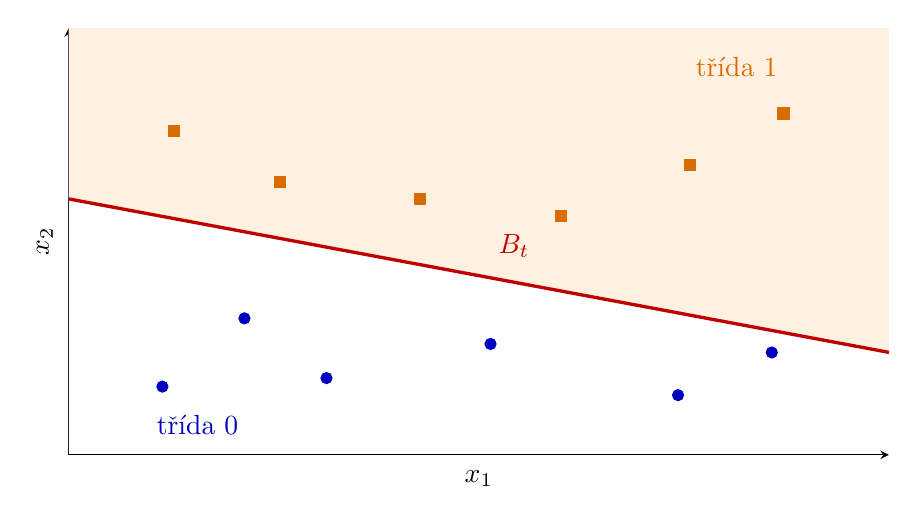
\begin{tikzpicture}
    \begin{axis}[
        width=12cm,height=7cm,
        xmin=0,xmax=7,ymin=0,ymax=5,
        axis lines=left,xlabel={$x_1$},ylabel={$x_2$},
        xtick=\empty,ytick=\empty,
        label style={font=\normalsize},
        every node/.style={font=\normalsize},
        clip=false
    ]
        \addplot[draw=none,fill=orange!12]
        coordinates{(0,3)(7,1.2)(7,5)(0,5)}\closedcycle;
        \addplot[red!75!black,very thick,domain=0:7]{3-0.257*x};
        \addplot[only marks,mark=*,blue!75!black]
        coordinates{(0.8,0.8)(1.5,1.6)(2.2,0.9)(3.6,1.3)(5.2,0.7)(6,1.2)};
        \addplot[only marks,mark=square*,orange!85!black]
        coordinates{(0.9,3.8)(1.8,3.2)(3,3)(4.2,2.8)(5.3,3.4)(6.1,4)};
        \node[red!75!black] at (axis cs:3.8,2.45){\(B_t\)};
        \node[blue!75!black] at (axis cs:1.1,0.35){třída \(0\)};
        \node[orange!85!black] at (axis cs:5.7,4.55){třída \(1\)};
    \end{axis}
\end{tikzpicture}
